\section{Air System Fans }\label{air-system-fans}

\subsection{Overview}\label{overview-002}

Four input objects (Fan:SystemModel, Fan:ConstantVolume, Fan:VariableVolume,
and Fan:OnOff) provide models for fans -- the prime movers in most of the air
loop and zonal air conditioning systems in EnergyPlus. The 
\emph{Fan:SystemModel} input object was added for version 8.7 with the intent
that it provide a single versatile input object that could eventually replace
Fan:ConstantVolume, Fan:VariableVolume, and Fan:OnOff. For these input objects,
EnergyPlus uses a simple polynomial-based curve-fit model to describe the
relation between the volume flow rate and the fan electric power, with no
explicit modeling of fan pressure rise. Consequently, duct-static-pressure
reset strategies can only be modeled using curves that have been specially
developed to approximate static reset.  For CAV and VAV central air-handling
systems, a fifth input object (Fan:ComponentModel) provides a simple
physics-based model for flow-dependent fan pressure rise and detailed models
for fan, belt, motor, and variable-frequency-drive efficiencies and energy use.
This latter input object provides the capability to analyze the effects of
duct-static-pressure reset strategies, as well as changes in fan system element
performance. All of these fan models calculate the fan energy usage, which is
often a large fraction of HVAC energy use and a significant portion of the
building energy consumption. They also calculate the temperature rise in the
air stream caused by the static pressure increase as the air goes through the
fan. If the motor and belt are in the air stream, waste heat from the motor and
belt also acts to raise the air stream temperature.

\subsection{Model}\label{model-000}

Each of the five fan models is a forward type: the model inputs describe the
fan characteristics and the conditions of the air at the fan inlet; the outputs
are the fan electrical power consumption and the conditions of the air at the
fan outlet. The model algorithms and data for Fan:ConstantVolume,
Fan:VariableVolume, Fan:OnOff and Fan:ComponentModel are contained in the
\emph{Fans.cc} and \emph{Fans.hh} files in EnergyPlus.  The source code for the
Fan:SystemModel added for version 8.7 is contained in the \emph{HVACFan.cc} and
\emph{HVACFan.hh} files.

\subsubsection{Inputs and Data}\label{inputs-and-data-000}
For the Fan:SystemModel model (added for version 8.7), the user describes the fan by entering values for the design pressure rise across the fan, the design volume flow rate, the design electric power consumption, and the fan motor efficiency. The user also needs to specify the fraction of the fan motor's waste heat that will enter the air stream (usually 0 or 1). If the fan is indoors, the name of a Zone and a fraction for the split between thermal radiation and convection can be entered so that the portion of fan motor waste heat that does not enter the air stream can be added to the thermal zone surrounding the fan. The user enters a choice for fan speed control method to be either Continuous (for VAV) or Discrete (for constant volume, on-off, two-speed, or multi-speed).  A performance curve or lookup table defined separately can be referenced by the fan to describe the variation in fan power as a function of flow rate. This curve is required for continuous speed control. However, for discrete speed control the user has the option of directly entering a power modification factor for each discrete speed and a curve is not necessary. For two- or multi-speed fans, the number of speeds is entered and pairs of values for the flow fraction and power fraction at each speed level are entered in increasing order. The design electric power consumption can be autosized using input values for one of three available scaling factors: fan total efficiency, electric power per unit flow rate, or electric power per unit flow rate per unit pressure.  Except for these sizing and control features, the fan (system) model itself is based on the original fan models (Fan:VariableVolume, Fan:OnOff, and Fan:ConstantVolume) and uses the same basic mathematical formulation.

For the Fan:ConstantVolume, Fan:VariableVolume, and Fan:OnOff models, the user describes the fan by entering values for the design pressure rise across the fan, the design volume flow rate, the fan total efficiency, and the fan motor efficiency. The user also needs to specify the fraction of the fan waste heat that will enter the air stream (usually 0 or 1). For the Fan:VariableVolume model, the user must also enter the coefficients of a 4\(^{th}\) order polynomial that relates the fan mass flow rate to the fan power consumption.The independent variable is the volumetric flow fraction; the dependent variable is the fan power part load ratio. For multi-speed fans, the user must enter a fan power ratio as a function of speed ratio performance curve name. Multi-speed fans can only be simulated in a parent object which allows multiple fan speeds (e.g., AirLoopHVAC:Unitary:Furnace:HeatCool, ZoneHVAC:PackagedTerminalAirConditioner, etc.). An optional efficiency curve may also be used when simulating multi-speed fans to adjust the fan total efficiency as the fan speed changes.

For the Fan:ComponentModel object, the user describes the fan in more detail, and also describes the duct system characteristics as seen by the fan. In particular, the user specifies a pressure rise curve with four coefficients that relates the fan total pressure rise to the volumetric flow through the fan, the duct-static-pressure set-point, and the static pressure of the spaces surrounding the ducts. If duct-static-pressure reset is used, the user enters a linear curve with two coefficients that relates the pressure set-point to the volumetric flow through the fan. For the fan itself, the user specifies the fan geometry (wheel diameter and outlet area), maximum efficiency, the Euler number corresponding to the maximum efficiency, the maximum dimensionless flow, the names of four curves with several coefficients that describe the variation of fan efficiency and dimensionless flow with the Euler number in the normal and stall operation regions of the fan, and a sizing factor (applied to the maximum flow through the fan). For the belt, the user specifies the maximum efficiency (or a curve with five coefficients that defines the maximum efficiency as a function of maximum fan shaft input power), three curves with three coefficients each that relate the belt part-load efficiency to belt fractional output torque, the motor/fan pulley diameter ratio, the belt output torque capacity, and a sizing factor (applied to the maximum output torque of the belt). For the motor, the user specifies the maximum efficiency (or a curve with three coefficients that define the maximum efficiency as a function of maximum belt input power), a curve with three coefficients that relate the motor part-load efficiency to motor fractional output power, and a sizing factor (applied to the maximum output power of the motor). For the variable-frequency-drive (VFD), the user specifies a curve with three coefficients that relate the VFD part-load efficiency to motor fractional input power or to motor fractional speed, and a sizing factor (applied to the maximum output power of the VFD).

\subsubsection{Control}\label{control}

The models must decide whether the fan is on or off. The primary on/off trigger is the fan availability schedule. This is an on/off schedule associated with each fan: a value of 1 indicates the fan is on; a value of 0 indicates the fan is off. The fan schedule can be overruled by flags set by system availability managers. If the flag \emph{TurnFansOn} is true, a zero fan schedule value will be overridden and the fan will be turned on. If the flag \emph{TurnFansOff} is true the fan will be forced off. The inlet air mass flow rate must be greater than zero for the fan to be on.

Generally the fan is a passive component: it accepts the mass flow on its inlet node, uses it in its calculations of energy consumption and temperature rise, and passes it to the outlet node. However the fan maximum and minimum airflow rates act as absolute limits on the airflow rate.

For multi-speed fans, the parent object determines the fan speed ratio (i.e., the selected speed of the fan motor) and uses this value to determine flow rate and electric power consumption.  For a Fan:SystemModel operating with the Discrete choice for speed control, the fan model determines the faction of time spent at the discrete speeds that bound it and will produce the average flow requested by the parent object.  Then the fan electric power consumption is determined for each speed level and combined using a time-weighted average.  For a fan operating with Continuous speed control and a fan modeled with the Fan:OnOff object, the electric power is evaluated using the power ratio performance curve at the (average) flow fraction requested by the parent object. 

\subsubsection{Simulation}\label{simulation}

For the \emph{Fan:SystemModel} model based on design electric power consumption, the fan's total efficiency is determined at the beginning of the simulation using:

\begin{equation}
{e_{tot,max}} = \frac{({\dot V_{design,max} \cdot \Delta P  } )}{{ \dot Q_{tot, design}}}
\end{equation}

For a fan with discrete speed control with more than one speed and input data for Speed \emph{x} Electric Power Fraction, the fan's total efficiency at each speed \emph{x} is determined and stored using:

\begin{equation}
{e_{tot,x}} = \frac {({f_{flow,x}} \cdot {\dot V_{design,max} \cdot \Delta P  } )}{( {f_{power,x}} \cdot { \dot Q_{tot, design}})}
\end{equation}

For a fan with discrete speed control and no data for the power fraction at a speed, the power performance curve (or table) is evaluated first using the flow fraction for the speed:

\begin{equation}
{f_{power,x}} =  {func_{power curve}}({f_{flow,x}})
\end{equation}

The fan model and EnergyPlus's modeling of flow at air system nodes is actually calculated using mass flow rates.  User input for design maximum volume flow rate is converted to a design mass flow rate using a design density of air that is adjusted for altitude above sea level and dry air at 20°C drybulb.

\begin{equation}
{\dot m_{design,max}} = {\dot V_{design, max}} \cdot  {\rho_{air,design}}
\end{equation}

For a fan with discrete speed control with more than one speed, the design mass flow rate at each speed is determined and stored using:

\begin{equation}
{\dot m_{design,x}} = {f_{flow,x}} \cdot {\dot V_{design,max}}
\end{equation}
\\
Simple (Single Speed) Fan Model

The following equations define the model for this fan:

\begin{equation}
{\dot Q_{tot}} = \dot m\cdot \Delta P/({e_{tot,max}}\cdot {\rho_{air}})
\end{equation}

\begin{equation}
{\dot Q_{shaft}} = {e_{motor}}\cdot {\dot Q_{tot}}
\end{equation}

\begin{equation}
{\dot Q_{toair}} = {\dot Q_{shaft}} + ({\dot Q_{tot}} - {\dot Q_{shaft}})\cdot {f_{motortoair}}
\end{equation}

\begin{equation}
{h_{out}} = {h_{in}} + {\dot Q_{toair}}/\dot m
\end{equation}

\begin{equation}
{w_{out}} = {w_{in}}
\end{equation}

\begin{equation}
{T_{out}} = PsyTdbFnHW({h_{out}},{w_{out}})
\end{equation}

Fan Model for Changing Flow Rates

The fan will operate at a flow fraction that is determined by other HVAC equipment in the air system.  A parent object will control the air flow rates and the fan flow fraction is defined as the ratio of the current mass flow rate divided by the design mass flow rate.

\begin{equation}
{f_{flow, cur}} = \frac{\dot m_{cur}}{\dot m_{design,max}}
\end{equation}

The determination of electric power consumed at a flow fraction depends on if the speed control method is discrete or continuous.

Discrete Speed Control 

For the \emph{Fan:SystemModel} using discrete speed control, with the number of fan speeds set at 1, and the flow fraction is less than one, then the fan will be modeled as cycling between "off" and "on" over the timestep.  The time fraction is equal to the flow fraction so that:
 
\begin{equation}
{RTF_{On}} = {f_{flow, cur}}
\end{equation}

\begin{equation}
{\dot Q_{tot,elec}} = {RTF_{On}} \cdot \left( \frac{\dot m\cdot \Delta P}{{e_{tot}}\cdot {\rho_{air}}}\right)
\end{equation}

Similarly, for two-speed and multi-speed fans, the current flow fraction will be used to find the run time fraction for each of the adjacent speed levels *x* and *x+1* that bracket the flow fraction such that

\begin{equation}
{f_{flow,x}} \leq {f_{flow, cur}} \leq {f_{flow,x+1}}
\end{equation}

The runtime fraction spent at each speed is determined using

\begin{equation}
{RFT_{x}} = \left( \frac{({f_{flow,x+1}} - {f_{flow, cur}} )}{({f_{flow,x+1}} - {f_{flow,x}})}  \right)
\end{equation}

\begin{equation}
{RFT_{x+1}} = \left( \frac{({f_{flow, cur}} - {f_{flow,x}} )}{({f_{flow,x+1}} - {f_{flow,x}})}  \right)
\end{equation}

The electric power consumption is calculated using the design mass flow rates and the total efficiency stored for each speed and combined using the runtime fraction at each speed.

\begin{equation}
{\dot Q_{tot,elec}} = {RTF_{x}} \cdot \left( \frac{\dot m_{design,x}\cdot \Delta P}{{e_{tot,x}}\cdot {\rho_{air}}}\right)  +  {RTF_{x+1}} \cdot \left( \frac{\dot m_{design,x+1}\cdot \Delta P}{{e_{tot,x+1}}\cdot {\rho_{air}}}\right)
\end{equation}

The temperature of the air stream leaving the fan is calculated as above using this result for total power. 

Continuous Speed Control

For the \emph{Fan:SystemModel} using Continuous speed control the flow fraction is used to evaluate the power performance modification factor which is defined in a separate curve or table.  

\begin{equation}
{f_{power,cur}} =  {func_{power curve}}({f_{flow,cur}})
\end{equation}

\begin{equation}
{e_{tot,cur}} = \frac {( { \dot m_{cur} \cdot \Delta P  } )}{( {f_{power,cur}} \cdot { \dot Q_{tot, design} \cdot \rho_{air}})}
\end{equation}


Fan:OnOff Fan Model


The on/off fan model is similar to the simple fan model with the exception that the on/off fan may cycle on and off during a simulation time step. The cycling rate of the fan is known as the run time fraction. The calculation of run time fraction accounts for the part-load losses of other equipment used in the HVAC system. A part-load factor (a.k.a. part-load ratio) is first calculated for the fan as the ratio of the actual operating mass flow rate to the maximum fan mass flow rate. The run time fraction is then calculated as the part-load factor divided by the part-load fraction. The part-load fraction is determined by other HVAC equipment in the simulation (Ref. DX coil) for use by this specific fan model.

\begin{equation}
  f_{flow} = \frac{\dot{m}}{\dot{m}_{max}}
\end{equation}

\begin{equation}
  RTF = \frac{f_{flow}}{PLF}
\end{equation}

The total fan power is then calculated as the maximum fan power multipled by the run time fraction.

\begin{equation}
{\mathop Q\limits^\cdot_{tot}} = RTF\left[ {\mathop m\limits^\cdot  \cdot \Delta P/\left( {{e_{tot}}\cdot {\rho_{air}}} \right)} \right]
\end{equation}

The remaining calculations are the same as those described in the simple single-speed fan mode.

Multi-Speed Fan Model

The model used to simulate a multi-speed fan relies on the general fan laws to correct for speed changes in the fan's motor and the corresponding change in fan power and fan total efficiency. Two performance curves are used to define the change in power and efficiency as shown below. The power ratio curve must be used to simulate a multi-speed fan. The power ratio curve modifies the fan power based on a change in fan speed according to the cubic fan law. Exponents other than 3 are allowed. The efficiency ratio curve is used to correct for changes in nominal efficiency at alternate fan speeds. If either or both of these curves are not provided, the ratio is assumed to be 1.

The power ratio term is evaluated using an exponent performance curve. The form of the exponent curve equation is shown below.

\begin{equation}
ExponentCurveOutput = C1 + C2*{x^{C3}}
\end{equation}

The exponent performance curve is used to evaluate the power ratio as a function of speed ratio (x in the equation above). For typical fan performance, coefficient C1 = 0 and coefficient C2 = 1. The exponent (C3) is typically equal to 3 (cubed fan law) but other values are allowed.

\begin{equation}
PowerRatio = f{\left( {{N_{ratio}}} \right)^n} = ExponentCurveOutput
\end{equation}

The efficiency ratio curve is a quadratic or cubic curve used to evaluate the efficiency ratio as a function of speed ratio (x in the following equation). The cubic equation form is shown below.

\begin{equation}
EfficiencyCurveOutput = C1 + C2{\left( x \right)^2} + C3{\left( x \right)^3}
\end{equation}

The curve coefficients are determine by correlating the normalized fan total efficiency (i.e., the actual fan total efficiency divided by the nominal fan total efficiency at a speed ratio of 1) to the speed ratio (i.e., the ratio of actual air flow rate through the fan to the maximum fan air flow rate).

\begin{equation}
EfficiencyRatio = f\left( {{N_{ratio}}} \right) = EfficiencyCurveOutput
\end{equation}

To account for the change in fan speed and to ensure that the run time fraction is accurately calculated, an adjustment to the previous calculation for run time fraction is made. This adjusts the calculated run time fraction to account for times when the fan speed has been reduced and the new speed is now considered the fan's maximum speed. The speed adjusted run time fraction is then used in the fan power calculation.

\begin{equation}
RTF = \frac{RTF}{N_{ratio}}
\end{equation}

\begin{equation}
{\mathop Q\limits^ \bullet_{tot}} = RTF\left[ {\frac{{\mathop m\limits^ \bullet  \Delta P}}{{{e_{tot}}{\rho_{air}}}}} \right]\left( {\frac{{PowerRatio}}{{EfficiencyRatio}}} \right)
\end{equation}

Each of the performance curves described above may be used to model the performance of a multi-speed fan motor, however, the power ratio curve must be used to envoke the multi-speed simulation. These curves are used when the fan is used in an HVAC system having multiple flow rates (i.e., different flow rates in cooling and heating mode). If an HVAC system operates at the same speed in either cooling or heating mode, these curves are not required. When these curves are not used, the associated ratio term in the equation above is assumed to be 1. The remaining calculations are identical to the simple single-speed fan model described above.

Variable Speed Fan Model

The model for the variable speed fan is similar to the simple single-speed fan model except for a part load factor that multiplies the fan power consumption.

\begin{equation}
{f_{flow}} = \dot m/{\dot m_{design}}
\end{equation}

\begin{equation}
{f_{pl}} = {c_1} + {c_2} \cdot {f_{flow}} + {c_3} \cdot f_{flow}^2 + {c_4} \cdot f_{flow}^3 + {c_5} \cdot f_{flow}^4
\end{equation}

\begin{equation}
{\dot Q_{tot}} = {f_{pl}}\cdot {\dot m_{design}}\cdot \Delta P/\left( {{e_{tot}}\cdot {\rho_{air}}} \right)
\end{equation}

The rest of the calculation is the same as for the simple fan.

\subsubsection{Nomenclature for Simple Models}\label{nomenclature-for-simple-models}

\({\dot Q_{tot}}\) ~is the fan power in watts;

\(\dot m\) is the air mass flow in kg/s;

\({\dot m_{design,max}}\) is the design (maximum) air flow in kg/s;

\(\Delta P\) is the fan design pressure increase in Pascals;

\({e_{tot}}\) ~is the fan total efficiency;

\({\rho_{air}}\) is the air density at standard conditions in kg/m\(^{3}\);

\({e_{motor}}\) ~is the motor efficiency;

\({\dot Q_{shaft}}\) is the fan shaft power in watts;

\({\dot Q_{toair}}\) is the power entering the air in watts;

\({N_{ratio}}\) is the ratio of actual fan flow rate (or speed) to maximum fan flow rate (or speed)

\({h_{in}},{h_{out}}\) ~are the inlet and outlet air stream specific enthalpies in J/kg;

\({w_{in}},{w_{out}}\) ~are the inlet and outlet air stream humidity ratios;

\({T_{out}}\) ~is the outlet air temperature in degrees C;

\(PsyTdbFnHW\) is the EnergyPlus psychrometric routine relating enthalpy and humidity ratio to temperature;

\({f_{flow}}\) is the flow fraction or part-load ratio;

\({f_{pl}}\) ~is the part load factor.

Component Fan Model

The Fan:ComponentModel object is based upon combining: modified forms of fan, belt, motor, and variable-frequency-drive (VFD) element models (Stein and Hydeman 2004); a simplified fan pressure rise model with distribution system leakage, duct static pressure, and conditioned space pressure control effects included (Sherman and Wray 2010); and a diagnostic-based simplified duct static-pressure reset (SPR) scheme for air-handling systems (Federspiel 2004, 2005).

Fan \emph{electric} power depends on fan \emph{air} power (product of the airflow through and pressure rise across the fan), mechanical efficiencies (fan and belt), and electrical efficiencies (motor and drive). For systems with variable flows, none of these parameters is constant and all are interrelated. For example, Figure~\ref{fig:example-fan-performance-maps-manufacturers} shows that fan efficiency strongly depends on fan flow \emph{as well as} pressure rise, although this is not obvious from the manufacturer's power and speed performance map (top left). Fan efficiency maps can be derived from the manufacturer's performance map using a commercially-available software-based data extraction tool such as DigitizeIt and by applying the following equation to the extracted data:

\({\eta_{fan}} = \frac{{\Delta {P_{fan}} \cdot {Q_{fan}}}}{{{H_{fan}}}}\) ~~~~~~~~~~~~~~~~~~~~~~~~~~~~~~~~~~~~~~~~~~~~~~~~~~~~~~~~~~~~~~~~~~~~~~~~~~~~~~~~~~~~ ()

where \textbf{Δ}\emph{P\(_{fan}\)}is the fan pressure rise (Pa); \emph{Q\(_{fan}\)} is the fan flow at standard conditions (m\(^{3}\)/s); and \emph{H\(_{fan}\)} is the fan shaft power (W). Fan speed values also can be derived from the manufacturer's performance map using a similar software-based data extraction tool.

Fan pressure rise must be sufficient to overcome the air-handling system pressure drop, which depends on duct static pressure, on duct and equipment leakage, and on pressure drops across duct and duct-like elements (e.g., dampers, fittings), coils, and filters that are connected to the fan. Duct and duct-like pressure drops increase approximately as the square of the flow through them. However, pressure drops across coils and filters behave differently: they are proportional to the flow raised to a power n, which can approach one for high-efficiency filters and wet coils (Liu et al. 2003, Trane 1999).

The relation between system pressure drop and flow defines what is commonly called a ``system curve''. When system characteristics change, such as when the duct static pressure set point is varied, a family of system curves results. The intersections of these curves with fan curves (e.g., power as a function of pressure rise and flow) on a pressure versus flow plot define one or more loci of unique fan operating points. Each of these points has an associated fan efficiency, power, and speed.

\begin{figure}[hbtp] % fig 208
\centering
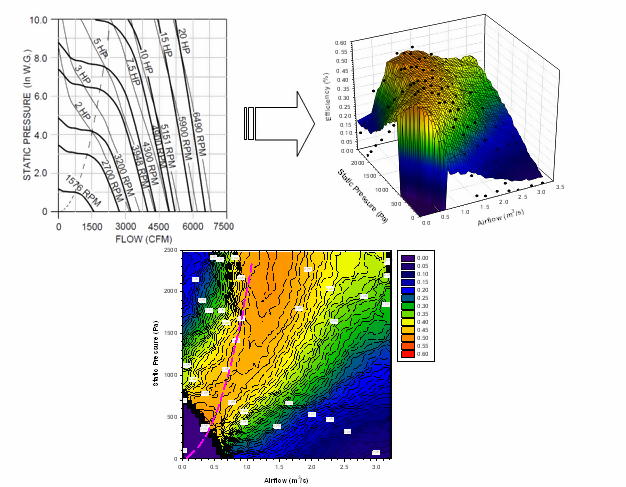
\includegraphics[width=0.9\textwidth, height=0.9\textheight, keepaspectratio=true]{media/image4888.png}
\caption{Example Fan Performance Maps - Manufacturer’s Data from Loren Cook Company, plus Derived Static Efficiency (Three-Dimensional and Contours) (Dashed Parabolic Curve is “Do Not Select Line”) \protect \label{fig:example-fan-performance-maps-manufacturers}}
\end{figure}

\emph{Fan Pressure Rise Model}: To calculate fan pressure rise based on flow through the fan, Sherman and Wray (2010) have developed a simple physics-based data-driven four parameter duct system model for the purpose of simulating its system curve. The embodiment of the model for a fixed outdoor air fraction that can be applied to constant- or variable-volume central air-handling systems is:

\(\Delta {P_{fan,tot}} = {A_{fpr}}Q_{fan}^2 + {B_{fpr}}Q_{fan}^{} + {C_{fpr}}Q_{fan}^{}\sqrt {{P_{sm}} - {P_o}} + {D_{fpr}}\left( {{P_{sm}} - {P_o}} \right)\) ~~~~~~~~~~~~~~~~~~~~~~~~~~~ ()

where \textbf{Δ}\emph{P\(_{fan,tot}\)} is the fan total pressure rise (Pa); \emph{Q\(_{fan}\)} is the fan flow at standard conditions (m\(^{3}\)/s); \emph{P\(_{sm}\)} is the duct static pressure set point (Pa); \emph{P\(_{o}\)} is the static pressure of the spaces surrounding the ducts (Pa); and \emph{A\(_{fpr}\)}, \emph{B\(_{fpr}\)}, \emph{C\(_{fpr}\)}, and \emph{D\(_{fpr}\)} are constant coefficients that represent different aspects of the fan pressure rise model as described below.

Fan static pressure rise is determined from the total pressure rise by subtracting the outlet velocity pressure:

\(\Delta {P_{fan}} = \Delta {P_{fan,tot}} - \frac{\rho }{2}{\left( {\frac{{{Q_{fan}}}}{{{A_{fan,out}}}}} \right)^2}\) ~~~~~~~~~~~~~~~~~~~~~~~~~~~~~~~~~~~~~~~~~~~~~~~~~~~~~~~~~~~~~~~~~~~~~~~~ ()

where \emph{A\(_{fan,out}\)} is the fan outlet area (m\(^{2}\)) and \emph{ρ} is the air density at the fan inlet (kg/m\(^{3}\)).

The first term in Equation looks like the common system curve in which the fan pressure rise is proportional to the square of the fan flow, but here it also depends implicitly on supply and return pressure losses, and in part on the fraction of the fan flow that is outdoor air (essentially ``leaks'' into and out of the return side of the system). Very often it is the only term considered, but that would only be correct with fixed-position dampers, no distribution system leakage, no linear resistance components, and no duct static pressure control.

The second term accounts for significant flow resistances in the system where the pressure difference is linearly proportional to the flow. Some filters and coils in the return may need this term to be adequately described. This term could be ignored if there are no linear components or if their pressure drops are very small compared to the other terms.

The third term, which depends on the fan flow and square root of the supply duct pressure \emph{P\(_{sm}\)}, accounts in part for air leakage from the supply system when damper positions are fixed or are changed independently of static pressure or fan flow. In this case, reducing or eliminating supply leakage results in a different system curve. This, however, might be only a minor ``correction'' to the simple system curves generally used. The third term is zero when VAV box dampers are modulated to control flow. Consequently, with variable-position supply dampers, reducing or eliminating supply leakage does not change the system curve.

The last term also accounts in part for leakage from the supply system when damper positions are fixed or are changed independently of static pressure or fan flow. This term indicates that the same fan pressure rise can be achieved by raising the duct pressure and closing dampers. The only change in the system in such a case is that the leakage flow may increase. The coefficient for this term is equal to one when the VAV box dampers are modulated to control flow. In both cases, this term may be the most important ``correction'' to the simple system curves generally used, especially at low flows.

In principle, especially for research applications of Energy Plus, the four individual fan pressure rise coefficients can be determined using duct design calculation tools for the entire system (e.g., Right-CommDuct, UNI-DUCT, Ductsize, Varitrane Duct Designer, T-Duct). In practice, however, especially for existing buildings, the necessary details may not be known sufficiently. In that case, one can make active measurements at different combinations of fan flows, outside air fractions, damper positions (if they are variable), and duct static pressures and then use non-linear system identification techniques to fit the data and determine the coefficients. If passive measurements can be made over a sufficiently long time so that a wide range of outside air settings, damper positions, and fan flows is obtained, one could instead regress the data to find all of the parameters in the equation. Unfortunately, there are no standardized test procedures available to draw upon, even though some standards appear to be related (e.g., ASHRAE 1999, 2008). Consequently, field test protocols need to be developed to determine the parameters for the new duct system model. These protocols then need to be integrated into standardized data collection and analysis tools such as Pacific Gas and Electric's ``Universal Translator'' tool. The California Energy Commission is funding such a project; data, procedures, and tools from this project will support the EnergyPlus implementation of the fan and duct system models described here.

\emph{SPR Model}: The model for duct-static-pressure reset (SPR) is based on a simple diagnostic procedure and a linear correlation between duct static pressure and supply fan airflow (Federspiel 2004, 2005). The diagnostic method involves measuring the static pressure at the duct static pressure sensor and the velocity pressure at the fan inlet (represents the fan flow) at multiple points over the fan's operating range, while the VAV box dampers attempt to control flow in response to a constant thermostat setpoint. The goal of the test is to define the lowest duct static pressure where all VAV boxes are still in control (dampers modulating). In the model, the correlation between \emph{P\(_{sm}\)} and \emph{Q\(_{fan}\)} is as follows for \emph{Q\(_{fan,min}\)} ≤ \emph{Q\(_{fan}\)} ≤ \emph{Q\(_{fan,max}\)}:

\({P_{sm}} = {P_{sm,\min }} + \left( {{P_{sm,\max }} - {P_{sm,\min }}} \right)*\frac{{\left( {{Q_{fan}} - {Q_{fan,\min }}} \right)}}{{\left( {{Q_{fan,\max }} - {Q_{fan,\min }}} \right)}} = {C_1} + {C_2}*{Q_{fan}}\) ~~~~~~~~~~~~~~~~~~~~~~~~ ()

Where

~\({C_1} = {P_{sm,\min }} - {C_2}*{Q_{fan,\min }}\) ~and \({C_2} = \frac{{\left( {{P_{sm,\max }} - {P_{sm,\min }}} \right)}}{{\left( {{Q_{fan,\max }} - {Q_{fan,\min }}} \right)}}\) ~~~~~~~~~~~~~~~~~~~~~~~~~~~~~~~ ()

For \emph{Q\(_{fan}\)} \textless{} \emph{Q\(_{fan,min}\)}, \emph{P\(_{sm}\)} = \emph{P\(_{sm,min}\)};for\emph{Q\(_{fan}\)} \textgreater{} \emph{Q\(_{fan,max}\)}, \emph{P\(_{sm}\)} = \emph{P\(_{sm,max}\)}

\emph{Fan Efficiency and Shaft Input Power Model}: A dimensionless parameter in the form of an Euler number can be used to simplify the description of fan static efficiency variations:

\(Eu = \frac{{\left( {\Delta {P_{fan}} * D_{fan}^4} \right)}}{{\left( {\rho * Q_{fan}^2} \right)}}\) ~~~~~~~~~~~~~~~~~~~~~~~~~~~~~~~~~~~~~~~~~~~~~~~~~~~~~~~~~~~~~~~~~~~~~~~~~~~~~~~~~~~~~ ()

where \textbf{Δ}\emph{P\(_{fan}\)} is the fan static pressure rise (Pa), \emph{D\(_{fan}\)} is the fan wheel outer diameter (m), \emph{ρ} is the air density at the fan inlet (kg/m\(^{3}\)), and \emph{Q\(_{fan}\)} is the fan flow at standard conditions (m\(^{3}\)/s). \emph{Eu} is nominally the ratio of pressure forces across the fan to inertial forces at the fan wheel exit.

By plotting the normalized fan static efficiency (\emph{static efficiency / maximum static efficiency}) versus the logarithm base 10 of the normalized Euler number (\emph{Eu} \emph{/} \emph{Eu} \emph{at maximum static efficiency}), the dimensionless performance of various fan sizes is very similar (as one might expect from the ``fan laws''), but so also is the dimensionless performance of different \emph{types} of fans (e.g., single-inlet plenum fans, double-inlet housed centrifugal fans, mixed flow fans, vane axial fans, fans with backward or forward curved blades). An example of this correlation for the ``normal operation'' (non-stall) and stall regions of eight fans is shown in Figure~\ref{fig:normalized-efficiency-curves-for-eight-fans}.

\begin{figure}[hbtp] % fig 209
\centering
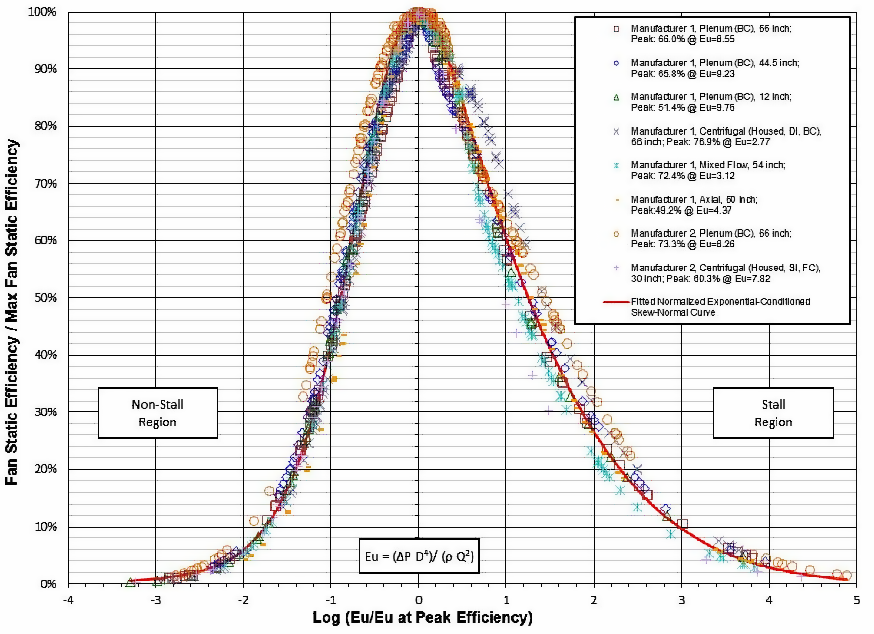
\includegraphics[width=0.9\textwidth, height=0.9\textheight, keepaspectratio=true]{media/image4895.png}
\caption{Normalized Efficiency Curves for Eight Fans in Dimensionless Space *(BC = backward curved, FC = forward curved; SI = single inlet, DI = double inlet)* \protect \label{fig:normalized-efficiency-curves-for-eight-fans}}
\end{figure}

This model uses a continuous function to represent the normalized fan efficiency (\emph{η\(_{fan}\)}) variation. The normalized exponential-conditioned skew-normal functional relationship is:

\begin{equation}
\frac{{{\eta_{fan}}({x_{fan}})}}{{{\eta_{fan,\max }}}} = \frac{{{e^{( - 0.5*Z_1^2)}}[1 + \frac{{{Z_2}}}{{\left| {{Z_2}} \right|}} \bullet erf\left( {\frac{{\left| {{Z_2}} \right|}}{{\sqrt 2 }}} \right)}}{{{e^{( - 0.5*Z_3^2)}}[1 + \frac{{{Z_3}}}{{\left| {{Z_3}} \right|}} \bullet erf\left( {\frac{{\left| {{Z_3}} \right|}}{{\sqrt 2 }}} \right)}}
\end{equation}

where

x\(_{fan}\) = log\(_{10}\)(Eu / Eu\(_{max}\))

Z\(_{1}\) = (x\(_{fan}\) - a\(_{fan}\)) / b\(_{fan}\);~ Z\(_{2}\) = ((e\(^{(c}\)fan\(^{*x}\)fan\(^{)}\)*d\(_{fan}\)*x\(_{fan}\)) - a\(_{fan}\)) / b\(_{fan}\);~ Z\(_{3}\) = -a\(_{fan}\) / b\(_{fan}\)

For conceptual design when only rough estimates are needed, a generic curve (also shown in Figure~\ref{fig:normalized-efficiency-curves-for-eight-fans}) can be used and then one only needs to know the maximum efficiency (\emph{η\(_{fan,max}\)}) and \emph{Eu} at that maximum (\emph{Eu\(_{max}\)}) to entirely model the fan efficiency and hence fan power. The dimensionless coefficients for the generic normalized fan efficiency curve are as follows:

\emph{a\(_{fan}\)} = -2.732094, \emph{b\(_{fan}\)} = 2.273014,\emph{c\(_{fan}\)} = 0.196344, \emph{d\(_{fan}\)} = 5.267518

In this case, the coefficient of determination R\(^{2}\) is 0.994. Also, the average and RMS differences between the efficiency values based on extracted data and the fitted generic curve are, respectively, about 0.5\% and 1.4\%; maximum differences are about ±9\%.

If more accuracy is needed for a specific fan, a similarly shaped curve can be developed for that fan (using extracted data, Equation , and least-squares regression techniques), segmented into normal operation and stall regions with specific coefficients fitted for each region. Figure~\ref{fig:example-normalized-efficiency-data-for-one} shows an example, using the data from Figure~\ref{fig:example-fan-performance-maps-manufacturers}.

\begin{figure}[hbtp] % fig 210
\centering
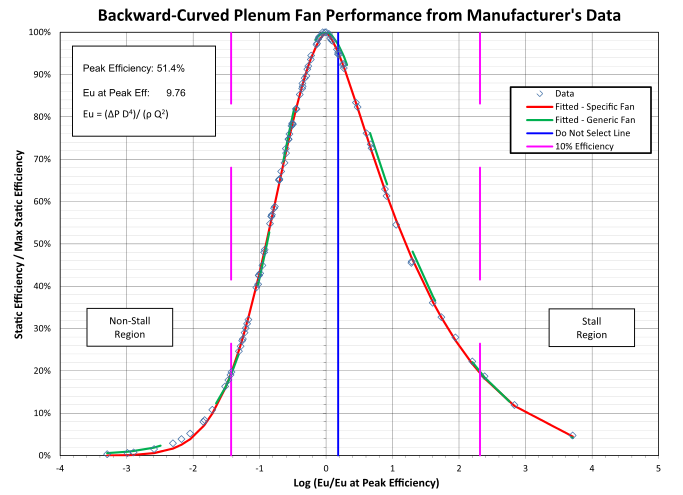
\includegraphics[width=0.9\textwidth, height=0.9\textheight, keepaspectratio=true]{media/image4897.svg.png}
\caption{Example Normalized Efficiency Data for One Fan \protect \label{fig:example-normalized-efficiency-data-for-one}}
\end{figure}

For this specific fan, the coefficients are:

% table 65
\begin{longtable}[c]{@{}lllll@{}}
\caption{Normalized Fan Efficiency Coefficients for Specific Backward-Curved Plenum Fan \label{table:normalized-fan-efficiency-coefficients-for}} \tabularnewline
\toprule 
Operating Region & a & b & c & d \tabularnewline
\midrule
\endfirsthead

\caption[]{Normalized Fan Efficiency Coefficients for Specific Backward-Curved Plenum Fan} \tabularnewline
\toprule 
Operating Region & a & b & c & d \tabularnewline
\midrule
\endhead

Normal (Non-Stall) & 0.072613 & 0.833213 & 0 & 0.013911 \tabularnewline
Stall & -2.354091 & 2.117493 & 0 & 2.753264 \tabularnewline
\bottomrule
\end{longtable}

In this case, the average and RMS differences between the efficiency values based on extracted data and fitted specific curve (R\(^{2}\) is 0.999) are, respectively, about -0.1\% and 0.3\%; maximum differences are about ±0.7\%. Field tests are especially needed to determine the coefficients for installed fans because fans are susceptible to ``system effects'' (e.g., inlet obstructions) that are not included in the manufacturer test data (AMCA 1990a).

To determine fan efficiency and fan shaft power at a particular time step, first calculate the fan pressure rise (\textbf{Δ}\emph{P\(_{fan}\)}) using the time step fan flow (\emph{Q\(_{fan}\)}) and Equation (and also using Equations and if there is SPR). Next, calculate \emph{Eu} using Equation and then \emph{x\(_{fan}\)} (log\(_{10}\) normalized \emph{Eu}), which is based on \emph{Eu} and the specified \emph{Eu\(_{max}\)} (\emph{Eu} at maximum efficiency) for the fan. The corresponding normalized efficiency (\emph{η\(_{fan}\)}(\emph{x\(_{fan}\)}) \emph{/ η\(_{fan,max}\)}) is obtained using Equation . The fan efficiency (\emph{η\(_{fan}\)}(\emph{x\(_{fan}\)})) therefore is:

\({\eta_{fan}}\left( {{x_{fan}}} \right) = {\eta_{fan,\max }}\left[ {\frac{{{\eta_{fan}}\left( {{x_{fan}}} \right)}}{{{\eta_{fan,\max }}}}} \right]\) ~~~~~~~~~~~~~~~~~~~~~~~~~~~~~~~~~~~~~~~~~~~~~~~~~~~~~~~~~~~~~~~~~ ()

The fan shaft input power (mechanical, W) is:

\({H_{fan}} = \frac{{\Delta {P_{fan}} \cdot {Q_{fan}}}}{{{\eta_{fan}}\left( {{x_{fan}}} \right)}}\) ~~~~~~~~~~~~~~~~~~~~~~~~~~~~~~~~~~~~~~~~~~~~~~~~~~~~~~~~~~~~~~~~~~~~~~~~~~~~~~~~~~~~~ ()

\emph{Fan Shaft Speed and Torque Modeling}: For rotating elements, power (\emph{H}) is the product of torque (\emph{τ}) and rotational speed (ω), or conversely, torque is power divided by rotational speed (\emph{τ = H / ω}).

The Stein and Hydeman variable-frequency-drive (VFD) component model correlates VFD efficiency as a linear function of VFD fractional output power (i.e., motor input power). Available data for about 50 drives from Saftronics were apparently used to develop their model, but those data represent VFD efficiency as a function of motor fractional speed (\emph{ω\(_{motor}\) / ω\(_{motor,max}\)}, or nominally, drive output frequency divided by maximum output frequency, if motor slip is ignored).

To make use of the available data, the Stein and Hydeman linear correlation must intrinsically make an assumption that motor speed and torque have some fixed relationship. Although not documented, their assumption might be the common belief that fractional torque (τ/ τ\(_{max}\)) for a motor is simply the square of its fractional speed. For fans serving duct systems with components such as filters and coils, with relatively low pressure drops elsewhere in the system, and for systems that have a non-zero controlled duct static pressure, this assumption may be inappropriate. Consequently, to make use of the available data and to avoid such assumptions, one needs to know the fraction of full speed at which fan components operate.

For the fan, dimensionless flow (\emph{φ}) can be defined as (ASHRAE 1993):

\(\varphi = \frac{{{Q_{fan}}}}{{{\omega_{fan}} \cdot D_{fan}^3}}\) ~~~~~~~~~~~~~~~~~~~~~~~~~~~~~~~~~~~~~~~~~~~~~~~~~~~~~~~~~~~~~~~~~~~~~~~~~~~~~~~~~~~~~~~~~~ ()

where \emph{ω\(_{fan}\)} is the fan speed (rad/s). This parameter can be calculated for each operating point on the fan manufacturer's performance map that represents fan speed as a function of flow and fan pressure rise. To simplify the data representation to a single curve (as we have done for fan efficiency), one can plot normalized dimensionless flow (dimensionless flow divided by maximum dimensionless flow, (\emph{φ}(\emph{x\(_{fan}\)}) \emph{/} \emph{φ\(_{max}\)}) as a function of the log base 10 of the normalized Euler (\emph{Eu}) parameter (\emph{x\(_{fan}\)}). Figure~\ref{fig:example-normalized-dimensionless-flow-data} shows an example plot derived from the manufacturer's data in Figure~\ref{fig:example-fan-performance-maps-manufacturers}.

\begin{figure}[hbtp] % fig 211
\centering
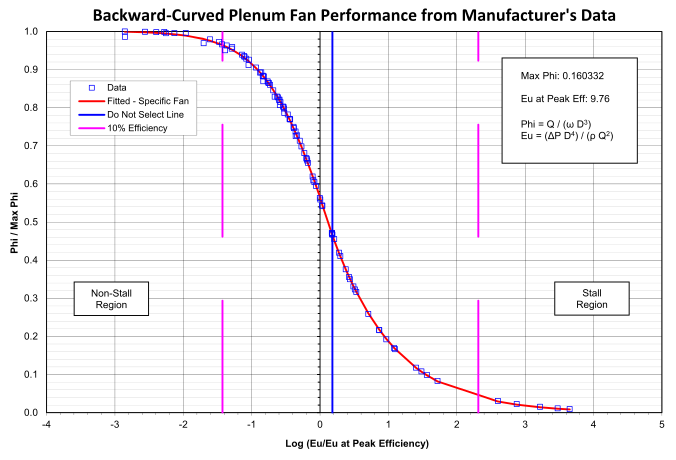
\includegraphics[width=0.9\textwidth, height=0.9\textheight, keepaspectratio=true]{media/image4901.svg.png}
\caption{Example Normalized Dimensionless Flow Data for One Fan \protect \label{fig:example-normalized-dimensionless-flow-data}}
\end{figure}

Equation describes the sigmoidal functional form for normalized \emph{φ}:

\(\frac{{\varphi \left( {{x_{fan}}} \right)}}{{{\varphi_{\max }}}} = ({A_{spd}} + {B_{spd}}/({(1 + {e^{\left[ {{{({C_{spd}} - {x_{spd}})} \mathord{\left/ {\vphantom {{({C_{spd}} - {x_{spd}})} {{D_{spd}}}}} \right. } {{D_{spd}}}}} \right]}})^{{E_{spd}}}})\) ~~~~~~~~~~~~~~~~~~~~~~~~~~~~~~~~~~~~~~~~~~~~ ()

where \emph{A\(_{spd}\)}, \emph{B\(_{spd}\)}, \emph{C\(_{spd}\)}, \emph{D\(_{spd}\)}, and \emph{E\(_{spd}\)} are coefficients for the fan. Separate sets of coefficients for the normal operation and stall regions can be specified. For the curve shown in Figure~\ref{fig:example-normalized-dimensionless-flow-data}, these coefficients are:

% table 66
\begin{longtable}[c]{@{}llllll@{}}
\caption{Dimensionless Flow Coefficients – Specific Backward-Curved Fan \label{table:dimensionless-flow-coefficients-specific}} \tabularnewline
\toprule 
Operating Region & A & B & C & D & E \tabularnewline
\midrule
\endfirsthead

\caption[]{Dimensionless Flow Coefficients – Specific Backward-Curved Fan} \tabularnewline
\toprule 
Operating Region & A & B & C & D & E \tabularnewline
\midrule
\endhead

Normal (Non-Stall) & 0 & 1.001423 & 0.123935 & -0.476026 & 1 \tabularnewline
Stall & 0 & 5.924993 & -1.916316 & -0.851779 & 1 \tabularnewline
\bottomrule
\end{longtable}

For a generic centrifugal fan with backward-curved blades, the coefficients are:

% table 67
\begin{longtable}[c]{@{}llllll@{}}
\caption{Dimensionless Flow Coefficients – Generic Backward-Curved Fan \label{table:dimensionless-flow-coefficients-generic}} \tabularnewline
\toprule 
Operating Region & A & B & C & D & E \tabularnewline
\midrule
\endfirsthead

\caption[]{Dimensionless Flow Coefficients – Generic Backward-Curved Fan} \tabularnewline
\toprule 
Operating Region & A & B & C & D & E \tabularnewline
\midrule
\endhead

Normal (Non-Stall) & -0.551396 & 1.551467 & -0.442200 & -0.414006 & 0.234867 \tabularnewline
Stall & 0.000608 & 0.586366 & 0.021775 & -0.063218 & 0.072827 \tabularnewline
\bottomrule
\end{longtable}

For any operating point of flow (\emph{Q\(_{fan}\)}) and fan pressure rise (\textbf{Δ}\emph{P\(_{fan}\)}), one can calculate the corresponding Euler number (\emph{Eu}) for the given fan, and then determine the corresponding normalized dimensionless flow (\emph{φ}(\emph{x\(_{fan}\)}) \emph{/} \emph{φ\(_{max}\)}) from the sigmoidal dimensionless flow function (Equation ). With \emph{φ}(\emph{x\(_{fan}\)}) \emph{/} \emph{φ\(_{max}\)} determined and knowing \emph{φ\(_{max}\)} for the fan, the dimensionless flow is:

\(\varphi \left( {{x_{fan}}} \right) = {\varphi_{\max }}\left[ {\frac{{\varphi \left( {{x_{fan}}} \right)}}{{{\varphi_{\max }}}}} \right]\) ~~~~~~~~~~~~~~~~~~~~~~~~~~~~~~~~~~~~~~~~~~~~~~~~~~~~~~~~~~~~~~~~~~~~~~~~~~~~~ ()

With \emph{φ}(\emph{x\(_{fan}\)}) determined, the fan rotational speed (rad/s) is:

\({\omega_{fan}} = \frac{{{Q_{fan}}}}{{\left( {\varphi ({x_{fan}}) * D_{fan}^3} \right)}}\) ~~~~~~~~~~~~~~~~~~~~~~~~~~~~~~~~~~~~~~~~~~~~~~~~~~~~~~~~~~~~~~~~~~~~~~~~~~~~~~~ ()

Fan shaft torque (N∙m), which the belt drive must supply to the fan shaft, is then:

\({\tau_{fan}} = \frac{{{H_{fan}}}}{{{\omega_{fan}}}}\) ~~~~~~~~~~~~~~~~~~~~~~~~~~~~~~~~~~~~~~~~~~~~~~~~~~~~~~~~~~~~~~~~~~~~~~~~~~~~~~~~~~~~~~~~~~~~~~~ ()

The fraction of full-load driven torque for the belt (\emph{τ\(_{fan}\) / τ\(_{belt,max}\)}), which is typically called ``belt load'', is thus \emph{τ\(_{fan}\)} divided by the belt torque capacity (\emph{τ\(_{belt,max}\)}). For a particular belt type and cross-section, belt torque capacity can be determined from manufacturer's information such as a shaft speed versus power chart.

Ignoring belt slip, motor shaft speed (\emph{ω\(_{motor}\)}, rad/s) can then be determined using the fan speed (\emph{ω\(_{fan}\)}) and the motor/fan pulley diameter ratio (\emph{D\(_{pulley,motor}\) / D\(_{pulley,fan}\)}), which is typically called the ``drive'' ratio:

\({\omega_{motor}} = \frac{{{\omega_{fan}}}}{{\left( {\frac{{{D_{pulley,motor}}}}{{{D_{pulley,fan}}}}} \right)}}\) ~~~~~~~~~~~~~~~~~~~~~~~~~~~~~~~~~~~~~~~~~~~~~~~~~~~~~~~~~~~~~~~~~~~~~~~~~~~~~~~~ ()

\emph{Belt, Motor, and Variable-Frequency-Drive Efficiency and Input Power Models -- Overview}: The models for belt drives, motors, and VFDs that Stein and Hydeman included in their air-handling system model represent maximum efficiency as a function of power input to the adjacent downstream component (e.g., the power input to a fan shaft by a belt drive), but they do not include part-load models. The part-load models are needed, because part-load efficiency for these components can fall off rapidly at low load (e.g., to zero at zero load) and many systems operate occasionally (and some much of the time) at low loads, in part because of current practices that result in substantial oversizing of components.

\emph{Belt Efficiency and Input Power Model:} Figure~\ref{fig:belt-maximum-efficiency-vs.-fan-shaft-power} shows three maximum efficiency (\emph{η\(_{belt,max}\)}) curves for belts (low, medium, and high) as a function of maximum fan shaft torque. This set of efficiency curves is based on belt drive loss data from AMCA Publication 203 (1990b), which reportedly is an aggregation of data from over 400 tests.

To determine \emph{η\(_{belt,max}\)} if data for a specific belt are not available, first use the maximum fan shaft input power (\emph{H\(_{fan,max}\)}) for the load spectrum to calculate the natural logarithm of belt power capacity:

\emph{x\(_{belt,max}\) =}ln(\emph{H\(_{fan,max}\)}) with \emph{H\(_{fan,max}\)} expressed in terms of hp~~~~~~~~~~~~~~~~~~~~~~~ ()

Then, use Equations and , along with a choice of low, medium, or high efficiency coefficients from Table~\ref{table:belt-maximum-efficiency-curve-coefficients}, to calculate \emph{η\(_{belt,max}\)}.

\begin{figure}[hbtp] % fig 212
\centering
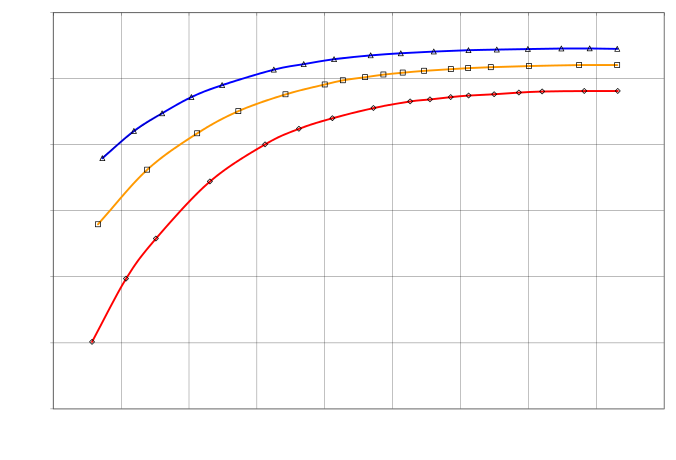
\includegraphics[width=0.9\textwidth, height=0.9\textheight, keepaspectratio=true]{media/image4907.svg.png}
\caption{Belt Maximum Efficiency vs. Fan Shaft Power Input \protect \label{fig:belt-maximum-efficiency-vs.-fan-shaft-power}}
\end{figure}

The quartic polynomial curves in Figure~\ref{fig:belt-maximum-efficiency-vs.-fan-shaft-power} and their coefficients are as follows:

\({\eta_{belt,\max ,\ln }} = {c_1} + {c_2} \cdot {x_{belt,\max }} + {c_3} \cdot x_{_{belt,\max }}^2 + {c_4} \cdot x_{_{belt,\max }}^3 + {c_5} \cdot x_{_{belt,\max }}^4\) ~~~~~~~~~~~~~~~~~~~ ()

% table 68
\begin{longtable}[c]{p{1.0in}p{1.0in}p{1.0in}p{1.0in}p{1.0in}p{1.0in}}
\caption{Belt Maximum Efficiency Curve Coefficients \label{table:belt-maximum-efficiency-curve-coefficients}} \tabularnewline
\toprule 
Efficiency Class (Loss) & c & c & c & c & c \tabularnewline
\midrule
\endfirsthead

\caption[]{Belt Maximum Efficiency Curve Coefficients} \tabularnewline
\toprule 
Efficiency Class (Loss) & c & c & c & c & c \tabularnewline
\midrule
\endhead

High (Low Loss) & -6.502E-2 & 2.475E-2 & -6.841E-3 & 9.383E-4 & -5.168E-5 \tabularnewline
Medium (Medium Loss) & -9.504E-2 & 3.415E-2 & -8.897E-3 & 1.159E-3 & -6.132E-5 \tabularnewline
Low (High Loss) & -1.422E-1 & 5.112E-2 & -1.353E-2 & 1.814E-3 & -9.909E-5 \tabularnewline
\bottomrule
\end{longtable}

The belt maximum efficiency is therefore:

\({\eta_{belt,\max }} = {e^{{\eta_{belt,\max ,\ln }}}}\) ~~~~~~~~~~~~~~~~~~~~~~~~~~~~~~~~~~~~~~~~~~~~~~~~~~~~~~~~~~~~~~~~~~~~~~~~~~~~~~~~~~ ()

The normalized \emph{part-load} belt efficiency model is provided to modify the maximum efficiency of the belt. This model is based on part-load data for belts in ACEEE's handbook on motor systems (Nadel et al. 2002). To determine the normalized belt efficiency at part-load (\emph{η\(_{belt}\)}(\emph{x\(_{belt}\)})/* η\(_{belt,max}\)\emph{), use the fan shaft (belt output) fractional torque (}x\(_{belt}\)* = \emph{τ\(_{belt}\)} / \emph{τ\(_{belt,max;}\) τ\(_{belt}\) = τ\(_{fan}\)}) as the belt fractional load in Equation or (select the equation for the region that contains \emph{x\(_{belt}\)}) and use coefficients from Table~\ref{table:belt-normalized-efficiency-curve-coefficients} that correspond to that region and the belt type: V-Belt or synchronous (toothed). Figure~\ref{fig:belt-normalized-efficiency-vs.-belt} shows a graphical representation of the curves defined by these equations and coefficients.

\begin{figure}[hbtp] % fig 213
\centering
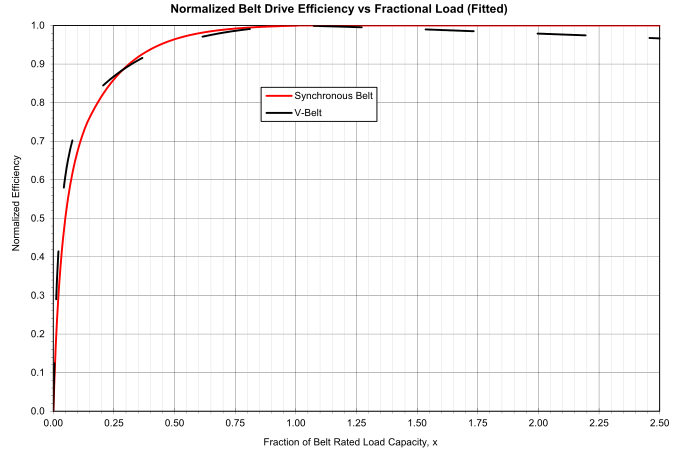
\includegraphics[width=0.9\textwidth, height=0.9\textheight, keepaspectratio=true]{media/image4910.svg.png}
\caption{Belt Normalized Efficiency vs. Belt Fractional Load) \protect \label{fig:belt-normalized-efficiency-vs.-belt}}
\end{figure}

The belt normalized (part-load) efficiency curves in Figure~\ref{fig:belt-normalized-efficiency-vs.-belt} for Regions 1 and 3 (single rectangular hyperbola type 2) and Region 2 (exponential decay), respectively, and their coefficients are as follows:

Region 1 (0 \textless{} = \emph{x\(_{belt}\)} \textless{} \emph{x\(_{belt,trans}\)}) and Region 3 (\emph{x\(_{belt}\)} \textgreater{} 1):

\(\frac{{{\eta_{belt}}({x_{belt}})}}{{{\eta_{belt,\max }}}} = \left[ {\frac{{{a_{belt}} \cdot {x_{belt}}}}{{{b_{belt}} + {x_{belt}}}}} \right] + {c_{belt}} \cdot {x_{belt}}\) ~~~~~~~~~~~~~~~~~~~~~~~~~~~~~~~~~~~~~~~~~~~~~~~~~~~~~~~~~~~~ ()

Region 2 (\emph{x\(_{belt,trans}\)} \textless{} = \emph{x\(_{belt}\)} \textless{} = 1):

\(\frac{{{\eta_{belt}}({x_{belt}})}}{{{\eta_{belt,\max }}}} = {a_{belt}} + {b_{belt}} \cdot {e^{\left( {{c_{belt}} \cdot {x_{belt}}} \right)}}\) ~~~~~~~~~~~~~~~~~~~~~~~~~~~~~~~~~~~~~~~~~~~~~~~~~~~~~~~~~~~~~~ ()

where x\(_{belt}\) = \(\tau\) \(_{belt}\) / \(\tau\) \(_{belt,max}\)

Belt efficiency therefore is:

\({\eta_{belt}}({x_{belt}}) = {\eta_{belt,\max }}\left[ {\frac{{{\eta_{belt}}({x_{belt}})}}{{{\eta_{belt,\max }}}}} \right]\) ~~~~~~~~~~~~~~~~~~~~~~~~~~~~~~~~~~~~~~~~~~~~~~~~~~~~~~~~~~~~~~~~~~ ()

Belt input power (mechanical, W) at the motor shaft is:

\({H_{belt}} = \frac{{{H_{fan}}}}{{{\eta_{belt}}({x_{belt}})}}\) ~~~~~~~~~~~~~~~~~~~~~~~~~~~~~~~~~~~~~~~~~~~~~~~~~~~~~~~~~~~~~~~~~~~~~~~~~~~~~~~~~~~~~~ ()

% table 69
\begin{longtable}[l]{@{}llllll@{}}
\caption{Belt Normalized Efficiency Curve Coefficients \label{table:belt-normalized-efficiency-curve-coefficients}} \tabularnewline
\toprule 
Belt Type & x\(_{belt,trans}\) & Region & a\(_{belt}\) & b\(_{belt}\) & c\(_{belt}\) \tabularnewline \midrule
\midrule
\endfirsthead

\caption[]{Belt Normalized Efficiency Curve Coefficients} \tabularnewline
\toprule 
Belt Type & x\(_{belt,trans}\) & Region & a\(_{belt}\) & b\(_{belt}\) & c\(_{belt}\) \tabularnewline \midrule
\midrule
\endhead

V-Belt & 0.167 & 1 & 0.920797 & 0.026269 & 0.151594 \tabularnewline
 & & 2 & 1.011965 & -0.339038 & -3.43626 \tabularnewline
 & & 3 & 1.037778 & 0.010307 & -0.026815 \tabularnewline
Synchronous & 0.137 & 1 & 0.982167 & 0.049135 & 0.158164 \tabularnewline
 & & 2 & 1.002134 & -0.531885 & -5.295707 \tabularnewline
 & & 3 & 1 & 0 & 0 \tabularnewline
\bottomrule
\end{longtable}

\emph{Motor Efficiency and Input Power Model:} Figure~\ref{fig:maximum-motor-efficiency-vs.-belt-power-input} shows three maximum efficiency (\emph{η\(_{motor,max}\)}) curves for motors (low, medium, and high) as a function of rated motor output power (belt input power). This set of efficiency curves is based on maximum efficiency data in DOE's MotorMaster+ database (2003) from about 800 tests. It is provided for use in the absence of manufacturer's data.

\begin{figure}[hbtp] % fig 214
\centering
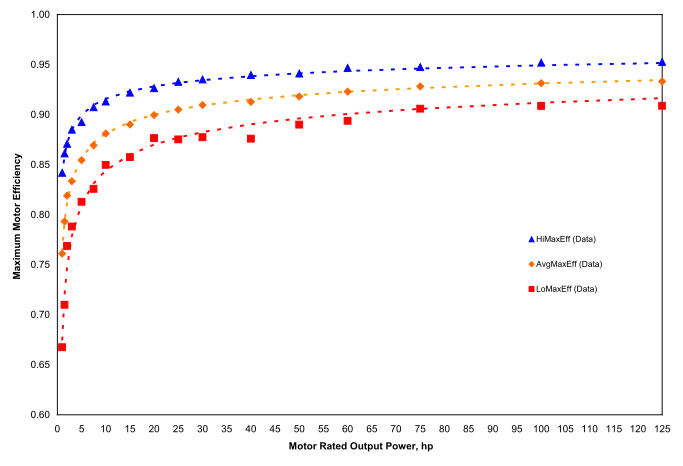
\includegraphics[width=0.9\textwidth, height=0.9\textheight, keepaspectratio=true]{media/image4917.svg.png}
\caption{Maximum Motor Efficiency vs. Belt Power Input (Motor Output) \protect \label{fig:maximum-motor-efficiency-vs.-belt-power-input}}
\end{figure}

To determine \emph{η\(_{motor,max}\)} if data for a specific motor are not available (e.g., as listed in Table~\ref{table:example-motor-normalized-efficiency-curve}), first use the maximum belt input power (\emph{H\(_{belt,max}\)}) for the load spectrum (multiplied by whatever oversizing factor may be desired) to calculate the natural logarithm of belt power capacity:

\emph{x\(_{motor,max}\) =}ln(\emph{H\(_{belt,max}\)}) with \emph{H\(_{belt,max}\)} expressed in terms of hp~~~~~~~~~~~~~~~~~~~~ ()

Then, use Equation , along with a choice of low, medium, or high efficiency coefficients from Table~\ref{table:motor-maximum-efficiency-curve-coefficients}, to calculate \emph{η\(_{motor,max}\)}.

The maximum motor efficiency curves in Figure~\ref{fig:maximum-motor-efficiency-vs.-belt-power-input} (single rectangular hyperbola type 1) and their coefficients are as follows:

\({\eta_{motor,\max }} = \left[ {\frac{{{a_{motor,\max }} \cdot {x_{motor,\max }}}}{{{b_{motor,\max }} + {x_{motor,\max }}}}} \right] + {c_{motor,\max }}\) ~~~~~~~~~~~~~~~~~~~~~~~~~~~~~~~~~~~~~~~~~~~~~ ()

% table 70
\begin{longtable}[c]{@{}llll@{}}
\caption{Motor Maximum Efficiency Curve Coefficients \label{table:motor-maximum-efficiency-curve-coefficients}} \tabularnewline
\toprule 
Case & a & b & c \tabularnewline
\midrule
\endfirsthead

\caption[]{Motor Maximum Efficiency Curve Coefficients} \tabularnewline
\toprule 
Case & a & b & c \tabularnewline
\midrule
\endhead

High-Efficiency & 0.196205 & 3.653654 & 0.839926 \tabularnewline
Mid-Efficiency & 0.292280 & 3.368739 & 0.762471 \tabularnewline
Low-Efficiency & 0.395895 & 3.065240 & 0.674321 \tabularnewline
\bottomrule
\end{longtable}

The normalized \emph{part-load} motor efficiency model is provided to modify the maximum efficiency of the motor. This model is based on part-load data for motors from DOE's MotorMaster+ database (2003). To determine the normalized motor efficiency at part-load (\emph{η\(_{motor}\)}(\emph{x\(_{motor}\)})/* η\(_{motor,max}\)\emph{), use the motor fractional power output (}x\(_{motor}\) = H\(_{belt}\)* / \emph{H\(_{belt,max}\)}) as the fraction of motor output power in Equation and use coefficients from Table~\ref{table:example-motor-normalized-efficiency-curve}, or for a specific motor, determined from DOE MotorMaster+ data or from manufacturer's data. Figure~\ref{fig:motor-normalized-efficiency-vs.-motor-load} shows a graphical representation of eight example curves defined by these equations and coefficients.

\begin{figure}[hbtp] % fig 215
\centering
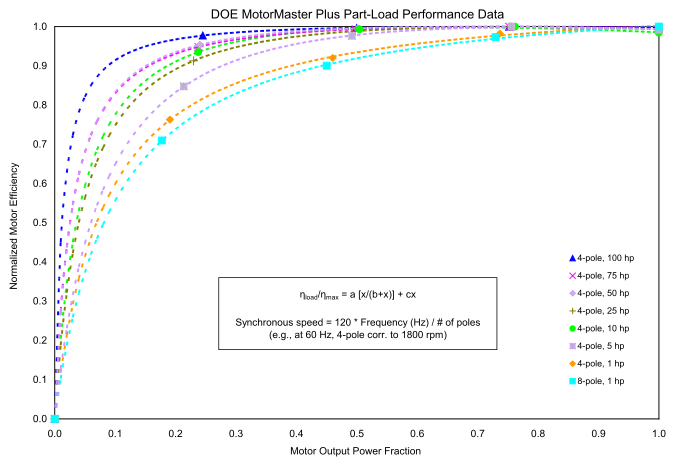
\includegraphics[width=0.9\textwidth, height=0.9\textheight, keepaspectratio=true]{media/image4919.svg.png}
\caption{Motor Normalized Efficiency vs. Motor Load Fraction \protect \label{fig:motor-normalized-efficiency-vs.-motor-load}}
\end{figure}

The example motor normalized efficiency curves (single rectangular hyperbola type 2) and their coefficients as a function of motor load fraction in Figure~\ref{fig:motor-normalized-efficiency-vs.-motor-load} are determined from DOE MotorMaster+ data and are as follows:

\(\frac{{{\eta_{motor}}({x_{motor}})}}{{{\eta_{motor,\max }}}} = \left[ {\frac{{{a_{PLmotor}} \cdot {x_{motor}}}}{{{b_{PLmotor}} + {x_{motor}}}}} \right] + {c_{PLmotor}} \cdot {x_{motor}}\) ~~~~~~~~~~~~~~~~~~~~~~~~~~~~~~~~~~~~~~~~~~~~ ()

% table 71
\begin{longtable}[c]{p{1.0in}p{1.0in}p{1.0in}p{1.0in}p{1.0in}p{1.0in}}
\caption{Example Motor Normalized Efficiency Curve Coefficients \label{table:example-motor-normalized-efficiency-curve}} \tabularnewline
\toprule 
Poles & Motor Rated Output (hp) & Maximum Efficiency & a\(_{Plmotor}\) & b\(_{Plmotor}\) & c\(_{Plmotor}\) \tabularnewline \midrule
\midrule
\endfirsthead

\caption[]{Example Motor Normalized Efficiency Curve Coefficients} \tabularnewline
\toprule 
Poles & Motor Rated Output (hp) & Maximum Efficiency & a\(_{Plmotor}\) & b\(_{Plmotor}\) & c\(_{Plmotor}\) \tabularnewline \midrule
\midrule
\endhead

8 & 1 & 0.6675 & 1.096694 & 0.097126 & 0.002011 \tabularnewline
4 & 1 & 0.7787 & 1.092165 & 0.08206 & -0.0072 \tabularnewline
 & 5 & 0.84 & 1.223684 & 0.08467 & -0.135186 \tabularnewline
 & 10 & 0.8745 & 1.146258 & 0.045766 & -0.110367 \tabularnewline
 & 25 & 0.8991 & 1.137209 & 0.050236 & -0.08915 \tabularnewline
 & 50 & 0.9129 & 1.088803 & 0.029753 & -0.064058 \tabularnewline
 & 75 & 0.9259 & 1.07714 & 0.029005 & -0.04935 \tabularnewline
 & 100 & 0.9499 & 1.035294 & 0.012948 & -0.024708 \tabularnewline
 & 125 & 0.9527 & 1.030968 & 0.010696 & -0.023514 \tabularnewline
\bottomrule
\end{longtable}

Motor efficiency therefore is:

\({\eta_{motor}}({x_{motor}}) = {\eta_{motor,\max }}\left[ {\frac{{{\eta_{motor}}({x_{motor}})}}{{{\eta_{motor,\max }}}}} \right]\) ~~~~~~~~~~~~~~~~~~~~~~~~~~~~~~~~~~~~~~~~~~~~~~~~~~~~~~~~~ ()

Motor input power (electrical, W) is:

\({H_{motor}} = \frac{{{H_{belt}}}}{{{\eta_{motor}}({x_{motor}})}}\) ~~~~~~~~~~~~~~~~~~~~~~~~~~~~~~~~~~~~~~~~~~~~~~~~~~~~~~~~~~~~~~~~~~~~~~~~~~~~~~~~~ ()

\emph{VFD Efficiency and Input Power Model:} For VFDs, published performance data are limited. Data from DOE (2008) suggest using a functional relation similar to that used for motors to represent VFD efficiency (\emph{η\(_{VFD}\)}) as a function of the fraction of full-load motor input power (\emph{x\(_{VFD}\) = H\(_{motor}\)} / \emph{H\(_{motor,max}\)}), as shown in Figure~\ref{fig:vfd-efficiency-vs.-fraction-of-motor-full}, or as a function of the fraction of full-load speed (\emph{x\(_{VFD}\) = ω\(_{motor}\) / ω\(_{motor,max}\)}), as shown in Figure~\ref{fig:vfd-efficiency-vs.-fraction-of-full-load}.

\begin{figure}[hbtp] % fig 216
\centering
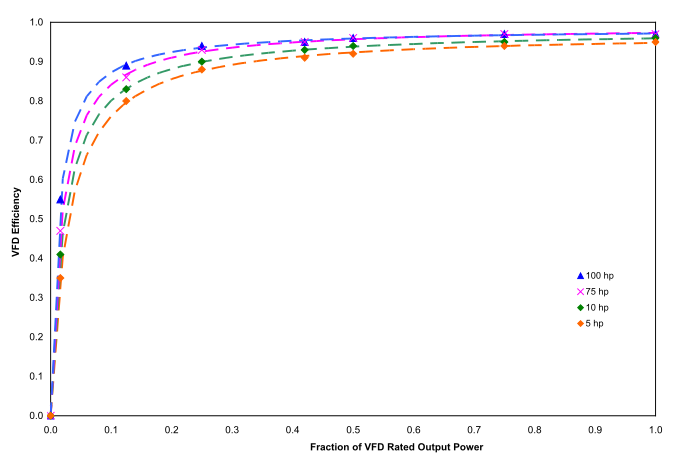
\includegraphics[width=0.9\textwidth, height=0.9\textheight, keepaspectratio=true]{media/image4923.svg.png}
\caption{VFD Efficiency vs. Fraction of Motor Full-Load Input Power (*Source: DOE 2008*) \protect \label{fig:vfd-efficiency-vs.-fraction-of-motor-full}}
\end{figure}

\begin{figure}[hbtp] % fig 217
\centering
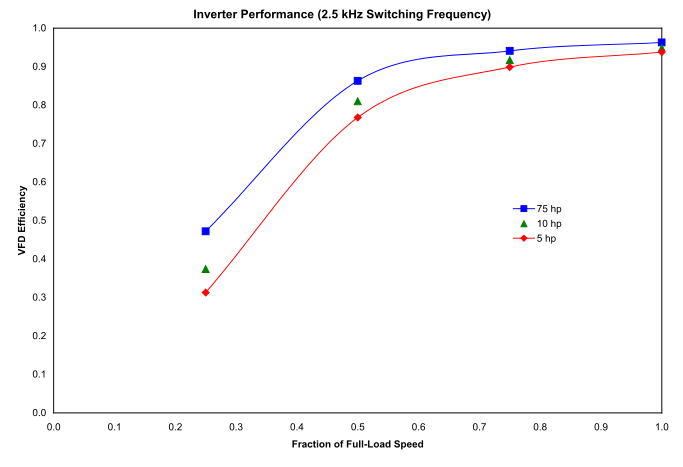
\includegraphics[width=0.9\textwidth, height=0.9\textheight, keepaspectratio=true]{media/image4924.svg.png}
\caption{VFD Efficiency vs. Fraction of Full-Load Motor Speed (*Courtesy of Saftronics*) \protect \label{fig:vfd-efficiency-vs.-fraction-of-full-load}}
\end{figure}

The performance curve (single rectangular hyperbola type 2) used here for VFD efficiency is:

\({\eta_{VFD}} = \left[ {\frac{{{a_{VFD}} \cdot {x_{VFD}}}}{{{b_{VFD}} + {x_{VFD}}}}} \right] + {c_{VFD}} \cdot {x_{VFD}}\) ~~~~~~~~~~~~~~~~~~~~~~~~~~~~~~~~~~~~~~~~~~~~~~~~~~~~~~~~~~~~~ ()

Example coefficients derived from the DOE data as a function of the fraction of full-load motor input power are listed in Table~\ref{table:example-vfd-efficiency-curve-coefficients}.

% table 72
\begin{longtable}[c]{@{}llll@{}}
\caption{Example VFD Efficiency Curve Coefficients \label{table:example-vfd-efficiency-curve-coefficients}} \tabularnewline
\toprule 
VFD Rated Output Power (hp) & a\(_{vfd}\) & b\(_{vfd}\) & c\(_{vfd}\) \tabularnewline \midrule
\midrule
\endfirsthead

\caption[]{Example VFD Efficiency Curve Coefficients} \tabularnewline
\toprule 
VFD Rated Output Power (hp) & a\(_{vfd}\) & b\(_{vfd}\) & c\(_{vfd}\) \tabularnewline \midrule
\midrule
\endhead

3 & 0.978856 & 0.034247 & -0.007862 \tabularnewline
5 & 0.977485 & 0.028413 & -0.002733 \tabularnewline
10 & 0.978715 & 0.022227 & 0.001941 \tabularnewline
20 & 0.984973 & 0.017545 & -0.000475 \tabularnewline
30 & 0.987405 & 0.015536 & -0.005937 \tabularnewline
50 & 0.987910 & 0.018376 & -0.001692 \tabularnewline
60 & 0.971904 & 0.014537 & 0.011849 \tabularnewline
75 & 0.991874 & 0.017897 & -0.001301 \tabularnewline
100 & 0.982384 & 0.012598 & 0.001405 \tabularnewline
>= 200 & 0.984476 & 0.009828 & -0.004560 \tabularnewline
\bottomrule
\end{longtable}

VFD input power (electrical, W) is:

\({H_{VFD}} = \frac{{{H_{motor}}}}{{{\eta_{VFD}}}}\) ~~~~~~~~~~~~~~~~~~~~~~~~~~~~~~~~~~~~~~~~~~~~~~~~~~~~~~~~~~~~~~~~~~~~~~~~~~~~~~~~~~~~~~~~~ ()

\emph{System Total Efficiency: T}he combined efficiency of the fan system components (i.e., fan, belt, motor, and VFD) is:

\({\eta_{TOTAL}} = {\eta_{fan}} \cdot {\eta_{belt}} \cdot {\eta_{motor}} \cdot {\eta_{VFD}}\) ~~~ \(\left( { = \frac{{{Q_{fan}} \cdot \Delta {P_{fan}}}}{{{H_{VFD}}}}} \right)\) ~~~~~~~~~~~~~~~~~~~~~~~~~~~~~~~~~~~~ ()

\emph{Heat Loss to Air}: To calculate the temperature rise from waste heat entering the air stream from the fan, belt, and motor, it is assumed that the user-specified ``motor in air fraction'' applies to the belt and motor but not to the VFD. The power ``lost'' to the air (W) is:

\({\dot Q_{toair}} = {H_{fan}} + \left( {{H_{motor}} - {H_{fan}}} \right) \cdot {f_{motortoair}}\) ~~~~~~~~~~~~~~~~~~~~~~~~~~~~~~~~~~~~~~~~~~~~~~~~~~~ ()

\subsection{References}\label{references-002}

AMCA. 1990a. ``Fans and Systems''. Publication 201-90. Arlington Heights, IL: Air Movement and Control Association International.

AMCA. 1990b. ``Field Performance Measurement of Fan Systems''. Publication 203-90. Arlington Heights, IL: Air Movement and Control Association International.

ASHRAE. 1993. HVAC 2 Toolkit: Algorithms and Subroutines for Secondary HVAC System Energy Calculations. Atlanta: American Society of Heating, Refrigerating and Air-Conditioning Engineers, Inc.

ASHRAE. 1999. ``ANSI/ASHRAE Standard 120 Method of Testing to Determine Flow Resistance of HVAC Ducts and Fittings''. Atlanta: American Society of Heating, Refrigerating and Air-Conditioning Engineers, Inc.

ASHRAE. 2008. ``ANSI/ASHRAE Standard 126 Method of Testing HVAC Air Ducts and Fittings''. Atlanta: American Society of Heating, Refrigerating and Air-Conditioning Engineers, Inc.

DOE. 2003. ``MotorMaster 4.0 User Guide''. U.S. Department of Energy, Industrial Technologies Program.

DOE. 2008. ``Energy Tips -- Motor: Motor Tip Sheet \#11''. U.S. Department of Energy, Industrial Technologies Program. June.

Federspiel, C. 2004. ``Detecting Optimal Fan Pressure''. Final Report of Federspiel Controls to the CEC Energy Innovations Small Grant Program. Grant \#: 02-03.

Federspiel, C. 2005. ``Detecting Critical Supply Duct Pressure''. ASHRAE Transactions, Vol. 111, Part 1. Atlanta: American Society of Heating, Refrigerating and Air-Conditioning Engineers, Inc.

Heredos, Francis P. 1987. Selection and Application of Multispeed Motors, IEEE Transactions on Industry Applications, Vol. 1A-23, No. 2, March/April.

Liu, M., D.E. Claridge, and S. Deng. 2003. ``An Air Filter Pressure Loss Model for Fan Energy Calculation in Air-Handling Units''. International Journal of Energy Research. Vol. 27, pp.~589-600.

Nadel, S., R.N. Elliot, M. Shepard, S. Greenberg, G. Katz, and A.T. de Almeida. 2002. ``Energy-Efficient Motor Systems: A Handbook on Technology, Program, and Policy Opportunities'' 2nd Edition. Washington, DC: American Council for an Energy Efficient Economy. p.188.

Sherman, M.H. and C.P. Wray. 2010. ``Parametric System Curves: Correlations Between Fan Pressure Rise and Flow for Large Commercial Buildings''. Lawrence Berkeley National Laboratory Report, LBNL-3542E.

Stein, J. and M.M. Hydeman. 2004. ``Development and Testing of the Characteristic Curve Fan Model''. ASHRAE Transactions, Vol. 110, Part 1. Atlanta: American Society of Heating, Refrigerating and Air-Conditioning Engineers, Inc.

Trane. 1999. ``Delta-Flo Coils: Data Catalog PL-AH-COIL-000-D-2-799''. LaCrosse, WI: The Trane Company. July.
